\documentclass[12pt]{article}
\usepackage[margin=2.5cm]{geometry}
\usepackage{enumerate}
\usepackage{amsfonts}
\usepackage{amsmath}
\usepackage{fancyhdr}
\usepackage{amsmath}
\usepackage{amssymb}
\usepackage{amsthm}
\usepackage{mdframed}
\usepackage{graphicx}
\usepackage{subcaption}
\usepackage{adjustbox}
\usepackage{listings}
\usepackage{xcolor}
\usepackage{booktabs}
\usepackage[utf]{kotex}

\definecolor{codegreen}{rgb}{0,0.6,0}
\definecolor{codegray}{rgb}{0.5,0.5,0.5}
\definecolor{codepurple}{rgb}{0.58,0,0.82}
\definecolor{backcolour}{rgb}{0.95,0.95,0.92}

\lstdefinestyle{mystyle}{
    backgroundcolor=\color{backcolour},
    commentstyle=\color{codegreen},
    keywordstyle=\color{magenta},
    numberstyle=\tiny\color{codegray},
    stringstyle=\color{codepurple},
    basicstyle=\ttfamily\footnotesize,
    breakatwhitespace=false,
    breaklines=true,
    captionpos=b,
    keepspaces=true,
    numbers=left,
    numbersep=5pt,
    showspaces=false,
    showstringspaces=false,
    showtabs=false,
    tabsize=1
}

\lstset{style=mystyle}

\pagestyle{fancy}
\renewcommand{\headrulewidth}{0.4pt}
\lhead{Hyungmo Gu}
\rhead{CSC209 Week 8 Notes}

\begin{document}
\title{CSC209 Week 8 Notes}
\author{Hyungmo Gu}
\maketitle

\section*{Processes 1 of 8}

\bigskip

\begin{itemize}
    \item Process Models
    \begin{itemize}
        \item Program
        \begin{itemize}
            \item The executable instructions of a program
            \item Source code
            \item Compiled machine code

            \begin{center}
            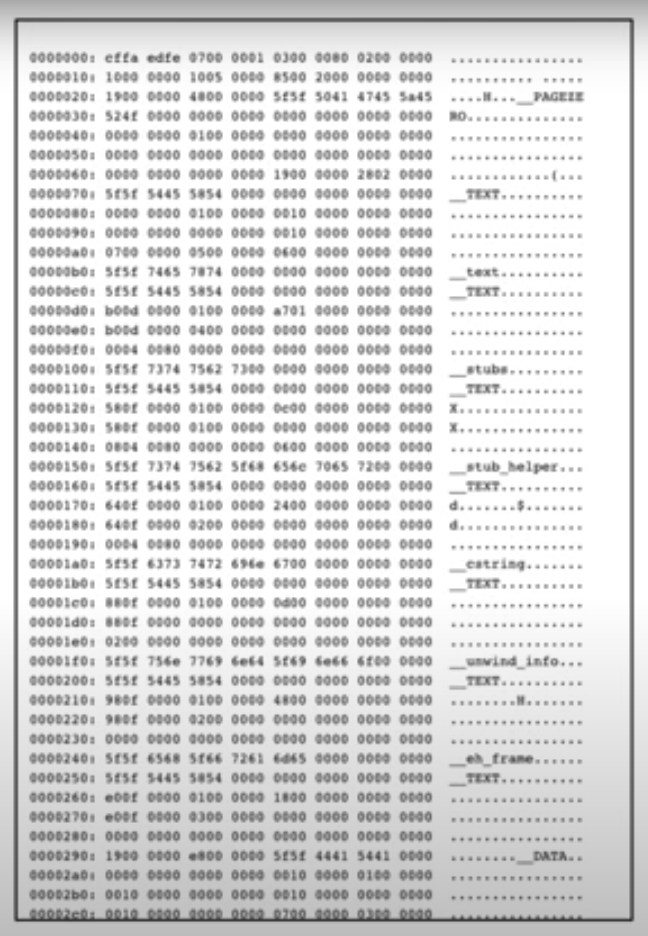
\includegraphics[width=0.5\linewidth]{images/week_8_notes_1_1.png}
            \end{center}

        \end{itemize}
        \item Process
        \begin{itemize}
            \item Running instance of program
            \item When program is ready for
        \end{itemize}

        \item State of Program
        \begin{itemize}
            \item
        \end{itemize}

        \item Top
        \item Three-state Process Management Model

        \begin{itemize}
            \item Running
            \item Ready
            \item Blocked
        \end{itemize}
    \end{itemize}
\end{itemize}

\end{document}